\chapter{Geometrische Algorithmen}

\begin{tcolorbox}[colframe=black!3!white]
  \textbf{Inhalt dieses Kapitels}:
  \tcblower{} 
  \begin{itemize}
    \item Plane-Sweep-Algorithmus
    \item Konvexe Hülle
    \item Kleinste einschließende Kugel
    \item Range Search
  \end{itemize}
\end{tcolorbox}

\section{Grundlegende Definitionen}

Wir nennen \( p \in \R^d \) einen \term{Punkt}\index{Punkt}. \( p\text{.}i \) stelle die \( i \)-te Komponente von \( p \) dar. Für \( d \in \left \{ 2,3 \right \} \) schreiben wir \( p\text{.}x \), \( p\text{.}y \), \( p\text{.}z \) statt \( p\text{.}1 \), \( p\text{.}2 \), \( p\text{.}3 \).

Für zwei Punkte \( a \), \( b \) definieren wir 
\begin{equation*}
  \overline{ab} \coloneqq \left \{ \alpha *a + (1-\alpha)*b : \alpha \in [0,1] \right \}
\end{equation*}
als das \term{Segment}\index{Segment} zwischen \( a \) und \( b \).

Ein \term{Polygon}\index{Polygon} ist eine Menge an Segmenten, gegeben als Punktemenge \( P = p_1, \dots, p_n \) mit \( p_i \in \R^d \), \( p_n = p_1 \). \( \overline{p_i, p_{i+1}} \) für \( i = 1,\dots,n-1 \) ist der \term{Umriss}\index{Polygon!Umriss} des Polygons.

Ist für alle \( a,b \in P \) auch \( \overline{ab} \in P \), so nennen wir \( P \) \term{konvex}\index{Polygon!konvex}.

\section{Streckenschnitte}

Bei diesem Problem sind \( n \) Strecken \( S = \left \{ s_1, \dots, s_n \right \} \) gegeben und wir wollen alle Schnittpunkte dieser, also \( \bigcup_{s,t \in S} s \cap t \) berechnen.

Naiv lassen sich diese Streckenschnitte in \( O(n^2) \) berechnen:

\begin{pseudocode}
  \textbf{foreach} \( \left \{ s,t \right \} \subseteq S \) \textbf{do} \\
  \phantom{\enskip} \textbf{if} \( s \cap t \neq \varnothing \) \textbf{then} output \( \left \{ s,t \right \} \)
\end{pseudocode}

Dieser Algorithmus ist für große Datenmengen offensichtlich zu langsam.

Idee ist nun, dass eine (waagerechte) \term{Sweep-Line}\index{Sweep-Line} von oben nach unten läuft. Dabei speichern wir Segmente, die \( l \) schneiden, und finden deren Schnittpunkte. Invariante ist, dass Schnittpunkte oberhalb von \( l \) korrekt ausgegeben wurden.

\subsection{Orthogonale Streckenschnitte}

Zuerst betrachten wir die Vereinfachung, dass nur orthogonale Segmente (also parallel zur \( x \)- oder \( y \)-Achse existieren).

\begin{pseudocode}
  \( T \coloneqq \left\langle  \right\rangle \) SortedSequence \textbf{of} Segment \\
  \textbf{invariant} \( T \) stores vertical segments intersecting \( l \) \\
  \( Q \coloneqq \text{sort}(\left\langle (y,s) : \exists \text{ hor-seg } s \text{ at } y \ \vee \ \exists \text{ ver-seg } s \text{ starting/ending at } y \right\rangle) \) \\
  \textbf{foreach} \( (y,s) \in Q \) in descending order \textbf{do} \\
  \phantom{\enskip} \textbf{if} \phantom{\enskip} \( s \) is ver-seg and \emph{starts} at \( y \) \textbf{then} \( T \).insert(\( s \)) \\
  \phantom{\enskip} \textbf{elif} \( s \) is ver-seg and \emph{ends} at \( y \) \textbf{then} \( T \).remove(\( s \)) \\
  \phantom{\enskip} \textbf{else} \phantom{\enskip} \textcolor{gray}{// horizontal segment \( s = \overline{(x_1,y)(x_2,y)} \)} \\
  \phantom{\enskip} \phantom{\enskip} \textbf{foreach} \( t = \overline{(x, y_1)(x,y_2)} \in T \) with \( x \in [x_1, x_2] \) \textbf{do} output \( \left \{ s,t \right \} \)
\end{pseudocode}

Hier sind \( T \) und \( Q \) die einzigen komplexen Datenstrukturen, die wir benötigen, also sortierte Listen an Segmenten (\( T \) geordnet nach \( x \)-Wert, \( Q \) nach \( y \)).

\texttt{insert} und \texttt{remove} gehen in \( O(\log n) \), die \texttt{rangeQuery} für ein Segment in \( O(\log n + k_s) \) (bei \( k_s \) Schritten mit horizontalem Segment \( s \)). Insgesamt haben wir also
\begin{equation*}
  O(n\log n + \sum_s k_s) = O(n\log n + k)\text{.}
\end{equation*}

\subsection{Verallgemeinerung}

Wir verallgemeinern jetzt den Spezialfall von oben, verwenden allerdings folgende Vereinfachungen: Es gebe keine horizontalen Segmente und Überschneidungen sind immer nur zwischen zwei Segmenten, nicht mehr. Außerdem soll es keine Überlappungen geben, die Anzahl an Schnitten zwischen zwei Segmenten ist also immer entweder \( 0 \) oder \( 1 \).

\begin{minipage}{.6\textwidth}
  \vspace*{1em}
  Wir verwenden wieder \( T \) als nach \( x \) geordnete Liste der Strecken, die \( l \) schneidet. Außerdem verwenden wir \emph{Ereignisse} --- diese sind Änderungen von \( T \), also das Starten und Enden von Segmenten sowie Schnittpunkte.

  Einen Schnittest müssen wir nur dann durchführen, wenn zwei Segmente an einem Ereignispunkt in \( T \) benachbart sind.
  \vspace*{1em}
\end{minipage}
\hfill
\begin{minipage}{.35\textwidth}
  \vspace*{1em}
  \begin{figure}[H]
    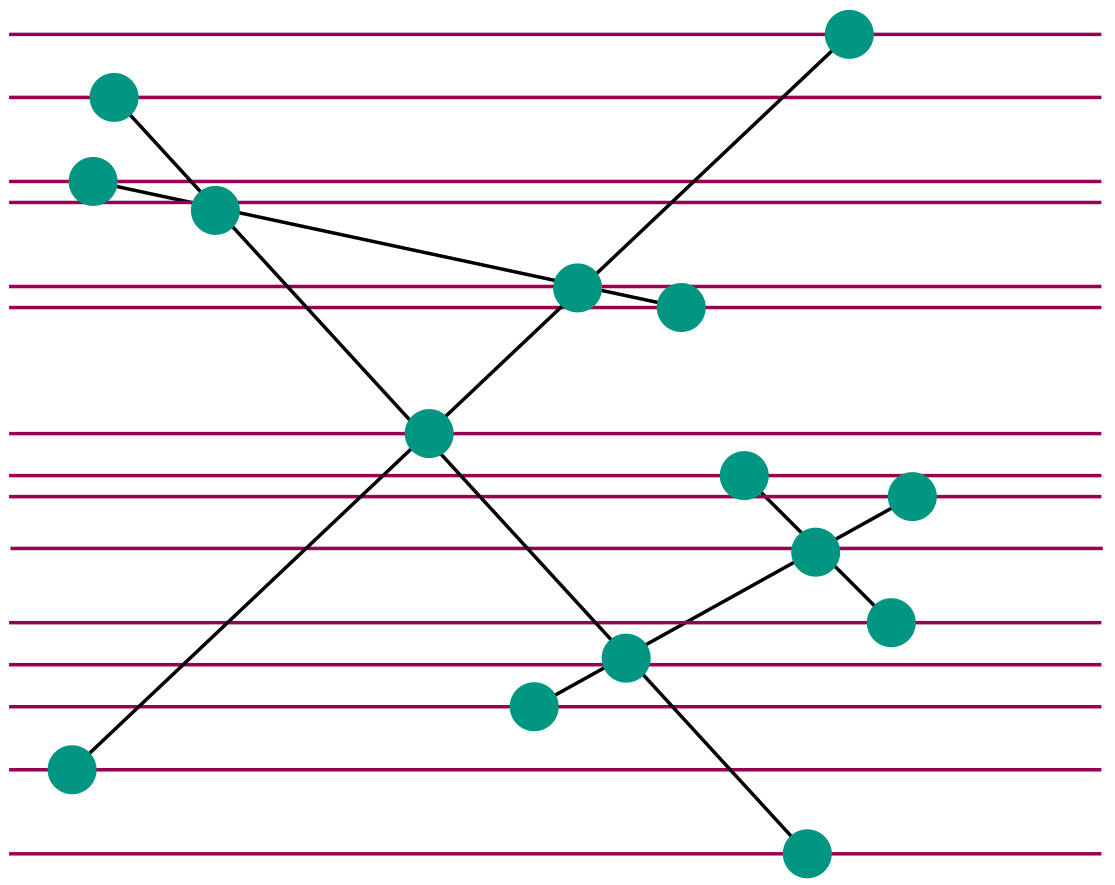
\includegraphics[width=\textwidth]{lineSweep}
    \caption{Die grünen Punkte stellen die Ereignisse dar. Außerdem ist \( l \) zum Zeitpunkt der Ereignisse dargestellt}
  \end{figure}
  \vspace*{1em}
\end{minipage}

Zur Implementierung brauchen wir nun einige Zusatzmethoden:

\begin{minipage}{.35\textwidth}
  \vspace*{1em}
  \textbf{\textsc{findNewEvent}} ermittelt, ob es einen Schnitt zwischen zwei Segmenten \( s \) und \( t \) gibt.
  \vspace*{1em}
\end{minipage}
\hfill
\begin{minipage}{.6\textwidth}
  \vspace*{1em}
  \begin{pseudocode}
    \textbf{\textsc{findNewEvent}}\( (s,t) \) \\
    \textbf{if} \( s \) and \( t \) cross at \( y' < y \) \textbf{then} \\
    \phantom{\enskip} \( Q \).insert(\( (y',\text{intersection},(s,t)) \))
  \end{pseudocode}
  \vspace*{1em}
\end{minipage}

\begin{minipage}{.36\textwidth}
  \vspace*{1em}
  Die Event-Handler werden kümmern sich um die Handhabung der drei möglichen Event-Types.
  \vspace*{1em}
\end{minipage}
\hfill
\begin{minipage}{.6\textwidth}
  \vspace*{1em}
  \begin{pseudocode}
    \textbf{\textsc{handleEvent}}\( (y, \text{\textbf{intersection}}, (a,b), T, Q) \) \\
    output(\( s \cap t \)) \\
    \( T \).swap(\( a \), \( b \)) \\
    \( \text{prev} \coloneqq \text{pred}(b) \) \\
    \( \text{next} \coloneqq \text{succ}(a) \) \\
    findNewEvent(prev, \( b \)) \\
    findNewEvent(\( a \), next)
  \end{pseudocode}
  \vspace*{1em}
\end{minipage}

\begin{minipage}{.475\textwidth}
  \vspace*{1em}
  \begin{pseudocode}
    \textbf{\textsc{handleEvent}}\( (y, \text{\textbf{start}}, s, T, Q) \) \\
    \( h \coloneqq T \).insert(\( s \)) \\
    \( \text{prev} \coloneqq \text{pred}(h) \) \\
    \( \text{next} \coloneqq \text{succ}(h) \) \\
    findNewEvent(prev, \( h \)) \\
    findNewEvent(\( h \), next)
  \end{pseudocode}
  \vspace*{1em}
\end{minipage}
\hfill
\begin{minipage}{.475\textwidth}
  \vspace*{1em}
  \begin{pseudocode}
    \textbf{\textsc{handleEvent}}\( (y, \text{\textbf{finish}}, s, T, Q) \) \\
    \( h \coloneqq T \).locate(\( s \)) \\
    \( \text{prev} \coloneqq \text{pred}(h) \) \\
    \( \text{next} \coloneqq \text{succ}(h) \) \\
    \( T \).remove(\( s \)) \\
    findNewEvent(prev, next)
  \end{pseudocode}
  \vspace*{1em}
\end{minipage}

Nun können wir den Algorithmus implementieren.

\begin{pseudocode}
  \( T \coloneqq \left\langle  \right\rangle \) SortedSequence \textbf{of} Segment \\
  \textbf{invariant} \( T \) stores relative order of segments intersecting \( l \) \\
  \( Q \coloneqq \) MaxPriorityQueue \\
  \( Q \coloneqq Q \cup \left \{ \left( \max\left \{ y,y' \right \}, \text{start}, s \right) : s = \overline{(x,y)(x',y')} \in S \right \} \) \\
  \( Q \coloneqq Q \cup \left \{ \left( \min\left \{ y,y' \right \}, \text{finish}, s \right) : s = \overline{(x,y)(x',y')} \in S \right \} \) \\
  \textbf{while} \( Q \neq \varnothing \) \textbf{do} \\
  \phantom{\enskip} \( (y,\text{type},s) \coloneqq Q \text{.deleteMax} \) \\
  \phantom{\enskip} handleEvent(\( y,\text{type},s,T,Q \))
\end{pseudocode}

Dieser Algorithmus benötigt \( O(n\log n) \) zur Initialisierung und \( O((n+k)\log n) \) für die Event-Schleife, insgesamt also \( O((n+k)\log n) \).

\section{Konvexe Hülle}

Wir werden uns in diesem Abschnitt mit dem folgenden Problem beschäftigen:

Gegeben sei eine Punktmenge \( P = \left \{ p_1, \dots, p_n \right \} \subset R^2 \). Gesucht ist ein konvexes Polygon \( C \) mit Eckpunkten \( \in P \), sodass alle Punkte von \( P \) in \( C \) liegen.

Zuerst sortieren wir \( P \) lexikographisch. Das bedeutet, dass
\begin{equation*}
  p > q \Leftrightarrow p\text{.}x > q\text{.}x \vee \left( p\text{.}x = q\text{.}x \wedge p\text{.}y > q\text{.}y \right)\text{.}
\end{equation*}

\begin{minipage}{.475\textwidth}
  \vspace*{1em}
  Wir berechnen ohne Einschränkung nur die obere Hülle, also die Hülle um die Punkte oberhalb von \( \overline{p_1 p_n} \).
  \vspace*{1em}
\end{minipage}
\hfill
\begin{minipage}{.475\textwidth}
  \vspace*{1em}
  \begin{figure}[H]
    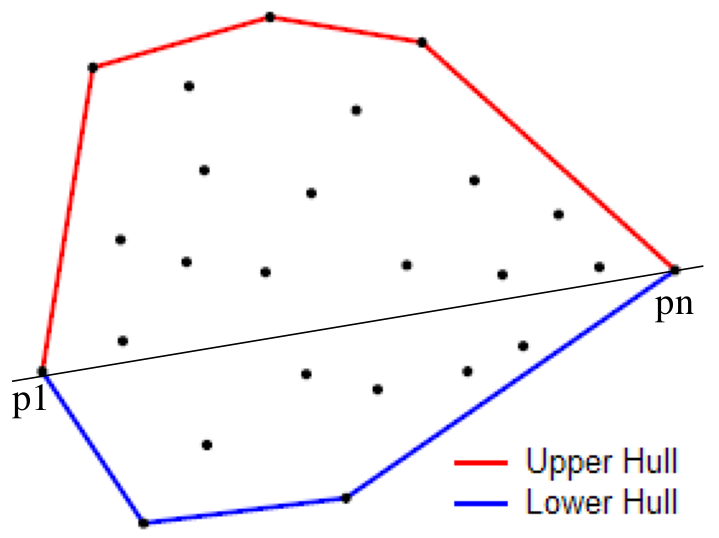
\includegraphics[width=\textwidth]{upperHull}
    \caption{Obere Hülle}
  \end{figure}
  \vspace*{1em}
\end{minipage}

Wir können beobachten, dass die obere Hülle ausschließlich Abbiegungen nach rechts macht (und die untere nur Abbiegungen nach links). Um damit arbeiten zu können müssen wir Abbiegungen definieren:

\begin{definition}[Abbiegung]
  Für eine Punktemenge \( P = \left \{ p_1, \dots, p_n \right \} \) ist eine \term{Abbiegung nach rechts}\index{Abbiegung} an Stelle \( i \) vorhanden, falls \( p_{i+1} \) rechts von \( \overline{p_{i-1}p_i} \) liegt.
\end{definition}

Das konstruieren der oberen Hülle nennt sich auch \term{Graham's Scan}\index{Graham's Scan}.\footnote{Graham 1972, Andrew 1979}

\begin{pseudocode}
  \textbf{\textsc{upperHull}}\( (p_1,\dots,p_n) \) \\
  \( L \coloneqq \left\langle p_n,p_1,p_2 \right\rangle \): Stack \textbf{of} Point \\
  \textbf{invariant} \( L \) is upper hull of \( \left\langle p_n,p_1,\dots,p_i \right\rangle \) \\
  \textbf{for} \( i \coloneqq 3 \) \textbf{to} \( n \) \textbf{do} \\
  \phantom{\enskip} \textbf{while} \( \neg \text{rightTurn}(L\text{.secondButlast},  L\text{.last}, p_i) \) \textbf{do} \( L\text{.pop} \) \\
  \phantom{\enskip} \( L \coloneqq L \circ \left\langle p_i \right\rangle \) \\
  \textbf{return} \( L \)
\end{pseudocode}

Der Algorithmus selbst läuft in \( O(n) \), weswegen das Sortieren dominiert und das ganze in \( O(n\log n) \) liegt.